% !TEX root = ../main.tex
% !TEX program = xelatex

\section{Übersicht}

\begin{frame}{How things have been done}
    \centering
    \Large{General Process - Flow Diagram}\\[2cm]
    \normalsize
    \begin{minipage}{.3\textwidth}
	\centering
	Perform a set of measurements in lab\\
	(Python)
    \end{minipage}
    \begin{minipage}{.02\textwidth}
	\centering
	$\rightarrow$
    \end{minipage}
    \pause
    \begin{minipage}{.3\textwidth}
	\
    \end{minipage}
    \begin{minipage}{.02\textwidth}
	\centering
	$\rightarrow$
    \end{minipage}
    \begin{minipage}{.3\textwidth}
    \centering
    Plot results\\
    (Python)
    \end{minipage}
\end{frame}


\begin{frame}{How things have been done}
    \centering
    \Large{General Process - Flow Diagram}\\[2cm]
    \normalsize
    \begin{minipage}{.3\textwidth}
	\centering
	Perform a set of measurements in lab \\
	(Python)
    \end{minipage}
    \begin{minipage}{.02\textwidth}
	\centering
	$\rightarrow$
    \end{minipage}
    \begin{minipage}{.3\textwidth}
	\centering
	Write results to .csv \\
	(done by hand)
    \end{minipage}
    \begin{minipage}{.02\textwidth}
	\centering
	$\rightarrow$
    \end{minipage}
    \begin{minipage}{.3\textwidth}
    \centering
    Plot results\\
    (Python)
    \end{minipage}
\end{frame}

\begin{frame}{Working on a solution}
    \Large{Problem: Usually quite large set of data}\\
    \normalsize
    For each measurement we have to
    \begin{itemize}
	\item Extract Parameters used (VCASN, ITHR) from the specific config
	    file
	    \pause
	\item Extract and analyze measurement data
	    \pause
	\item Write that information into a csv file for further analysis
	    \pause
    \end{itemize}
    \Large{Approach}\\
    \normalsize
    Simplyfying the process by writing a script that
    \begin{itemize}
	\item Extracts the \textbf{timestamp} for each measurement and properly
	    relates the .cfg to the .dat files
	    \pause
	\item performes analysis on ALL of the measurement data at once
	    \pause
	\item writes result to a csv file
    \end{itemize}
\end{frame}

\begin{frame}[fragile]{Scripting in Bash}
\small
ScanConfig\_\textbf{200121\_193551}.cfg \\
ScanConfig\_\textbf{200121\_193951}.cfg \\
ThresholdScan\_\textbf{200121\_193551}.dat \\
ThresholdScan\_\textbf{200121\_193951}.dat \\
\pause
\begin{lstlisting}

for i in $(ls $PATHTOFILES | grep '.dat'); do
#Extract Timestamp
TIMESTAMP=$(echo $i | tail -c 18 | head -c 13)
CONFIG="ScanConfig_$TIMESTAMP.cfg"

#Then extract Parameters from config file (Later add VBB)
VCASN=$(cat $PATHTOFILES$CONFIG | grep 'VCASN' | awk -F ' ' '{print $2}' | head -1)
ITHR=$(cat $PATHTOFILES$CONFIG | grep 'ITHR' | awk -F ' ' '{print $2}')

TRSH=$(./thresh.py $PATHTOFILES$i)

# Write to csv file
printf '%s\n' "$TIMESTAMP" "$VCASN" "$ITHR" "$TRSH" | paste -sd ',' >> output.csv
done
\end{lstlisting}
\pause
\begin{minipage}{.2\textwidth}
    \begin{figure}[H]
	\centering
	
\includegraphics[width=.5\textwidth]{Arrow2.png}
    \end{figure}
\end{minipage}
\begin{minipage}{.79\textwidth}
\begin{lstlisting}

Timestamp,VCASN,ITHR,Threshold [DAC]
200121_193551,47,51,13.60355155825141
200121_193951,47,60,15.953068558715911
...
\end{lstlisting}
\end{minipage}
\end{frame}

\begin{frame}[fragile]{Plotting}
    \Large{New Problem}\\
    \normalsize
    Data is not ordered, and the csv contains multiple entries for the same
    values of VCASN and ITHR \\
    \pause
    $\rightarrow$ When doing plots, formerly used hardcoding\\[.5cm]
    \pause
    \Large{Approach}\\
    \normalsize
    Write a "sorting" algorithm, that automatically identifies the ranges chosen
    for VCASN and ITHR. \\
    \begin{minipage}{.49\textwidth}
    \begin{lstlisting}
Timestamp,VCASN,ITHR,Threshold [DAC]
200323_134855,53,51,6.725833998523066
200323_135218,53,60,8.186236372633545
200323_135541,53,70,9.833234746846962
200323_132837,50,51,9.335578330893117
200323_133200,50,60,11.202496464178642
200323_133523,50,70,13.211766207119839
    \end{lstlisting}
\end{minipage}
\begin{minipage}{.04\textwidth}
    \centering
    $\rightarrow$
\end{minipage}
\begin{minipage}{.45\textwidth}
    \begin{lstlisting}
VCASN = array([50,53])
ITHR = array([51,60,70])
    \end{lstlisting}
\end{minipage}
\end{frame}

\begin{frame}[fragile]{plotting}
    \begin{lstlisting}

VCASN, ITHR, TRSH = np.loadtxt(csv, skiprows=1, usecols=(1,2,3), delimiter=",", unpack=True)

def getValues(array):
    #Create a temporary list
    temp = []
    #Write each unique entry into the temporary list
    for i in array:
        if i in temp: continue
        else: temp.append(i)
    #Since the array of values in this case is quite small, we can use temp.sort
    temp.sort()
    output = np.ndarray((len(temp)),dtype=int)
    for i in range(len(temp)):
        output[i] = int(temp[i])
    return output

VCASN_0 = getValues(VCASN)
ITHR_0 = getValues(ITHR)

##### Implement sorting algorithm #####
Threshold = np.ndarray((len(VCASN_0),len(ITHR_0)))
for i in range(len(VCASN_0)):
    for j in range(len(ITHR_0)):
        Threshold[i,j] = TRSH[(VCASN == VCASN_0[i]) & (ITHR == ITHR_0[j])]
#######################################

    \end{lstlisting}
\end{frame}

\begin{frame}{Results for 0 V Back Bias}
    \begin{minipage}{.49\textwidth}
    \begin{figure}[H]
	\centering
	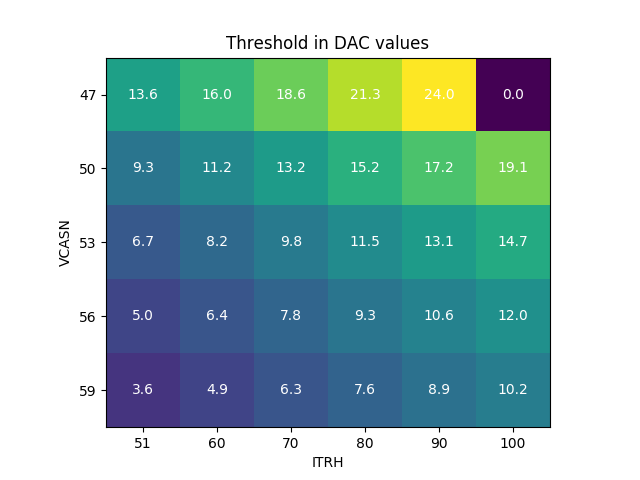
\includegraphics[width=\textwidth]{../bb0_Heatmap.png}
    \end{figure}
    \end{minipage}
    \begin{minipage}{.49\textwidth}
    \begin{figure}[H]
	\centering
	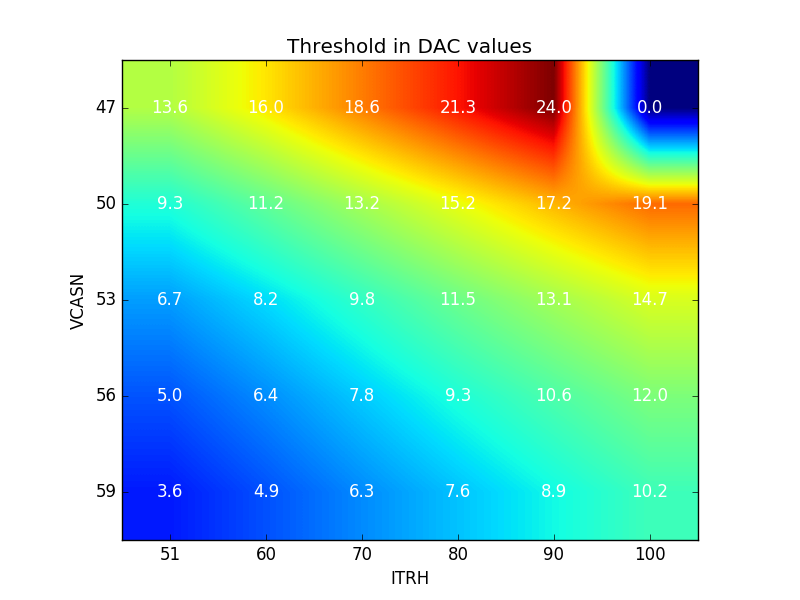
\includegraphics[width=\textwidth]{../bb0_Heatmap_soft.png}
    \end{figure}
    \end{minipage}\\[.5cm]
    \tiny
    Note: Value for VCASN = 47 and ITHR = 100 is faulty, due to a premature
    stop of the measurement after about 7\% of the injections.
    Threshold calculation fails there.
\end{frame}

\begin{frame}{Results for 3 V Back Bias}
    \begin{minipage}{.49\textwidth}
    \begin{figure}[H]
	\centering
	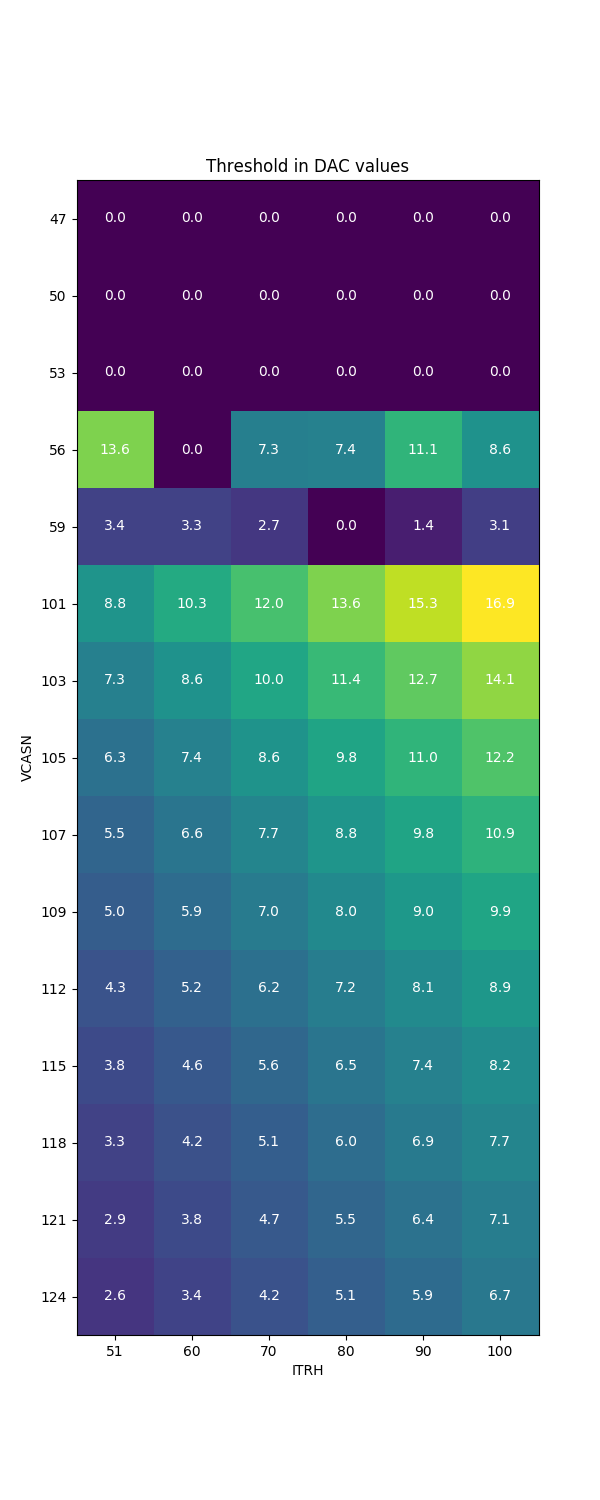
\includegraphics[width=3.5cm]{../bb3_Heatmap.png}
    \end{figure}
    \end{minipage}
    \begin{minipage}{.49\textwidth}
    \begin{figure}[H]
	\centering
	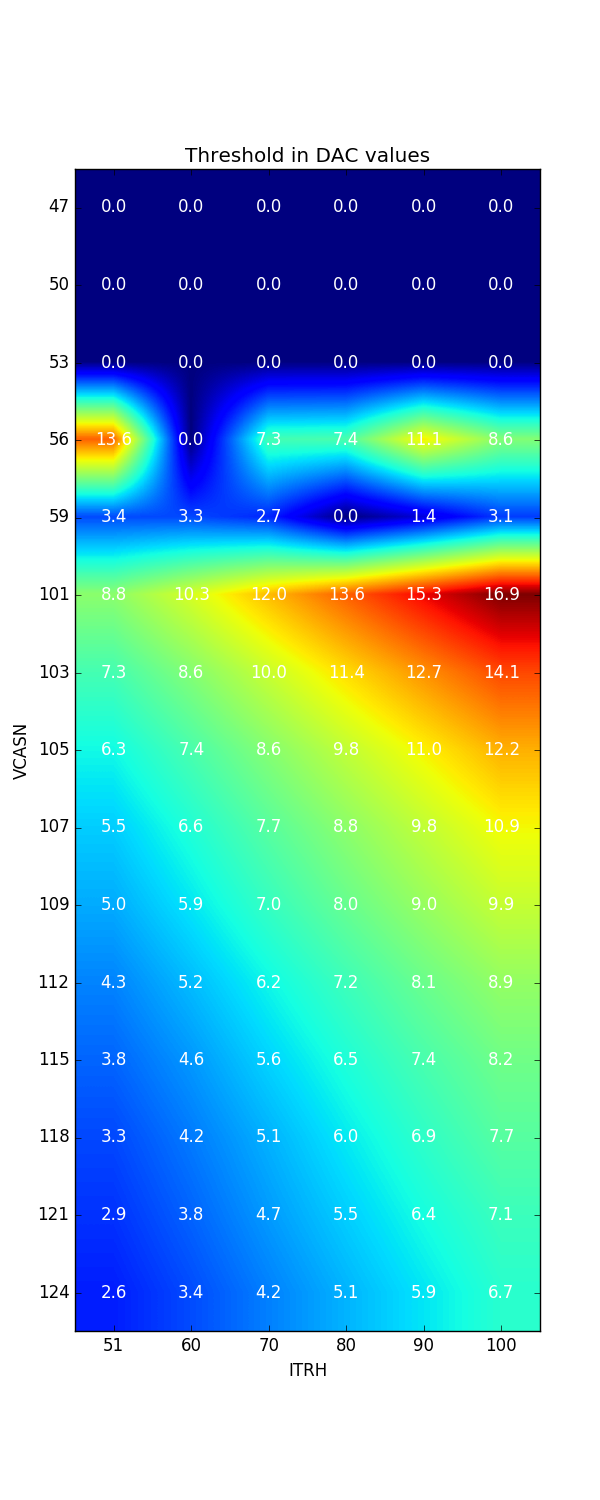
\includegraphics[width=3.5cm]{../bb3_Heatmap_soft.png}
    \end{figure}
    \end{minipage}
\end{frame}

\begin{frame}
    \Large For the future \\[.5cm]
    \normalsize Let the bash script...
    \begin{itemize}
	\item Include Errors
	    \pause
	\item Automatically detect faulty runs
	    \pause
	\item Work on different kinds of scans (NOISEOCC etc.)\\[1cm]
    \end{itemize}
    \pause
    \centering \huge \color{blue!30!black} \textbf{Thank you!}
\end{frame}
